\chapter{Experiments}
\label{ch:testing}

This section is divided into two main section -- one describes used datasets in the experiments, the other provides an implementation of functions I have written for the testing.

\section{Datasets}
\label{sec:expDatasets}

\subsection*{SCUT-CTW1500 Dataset}

SCUT-CTW1500 dataset contains exactly 1500 images of real-world, scene text in English language. Sample images can be seen in Figure \ref*{Im:Dctw}. The key feature of this dataset is that each image contains horizontally aligned text, multioriented text and curved text. There are cases where the curvature is only slight and cases where text forms a circle with letter upside down. Recognizing multi-oriented and curved text is more of a challenge than pure horizontal text. This dataset is split to train and test data. Two thirds of dataset thus one thousand images for training and five hundred for testing. According to the description of this dataset on relevant GitHub repository dataset was manually labeled and lately corrected, therefore labels seem to be very accurate. However for example ground truth for image 1313.jpg misses all occurences of letter I, as the depicted font was probably misread.\cite{ctw,ctw2}

The ground truth for train data are in XML format and each file carries information about the file name of respective image file, text information -- i.e., words in a text line, 14 coordinates of a bounding polygon and coordinates, height and width of a circumscribed rectangle. Later the authors added coordinates of center point of each English letter to be used as detection ground truth. The ground truth of test data is in simple text file (TXT) and contains only 14 coordinates of the bounding polygon and a text which is within that region. There is a minor issue with labels that it usually contains a full text line with multiple words and coordinates are not assigned to individual words but to text region as whole. Most end-to-end system detect words rather than groups of corresponding words. This fact needs to be taken into account when evaluating results.

\begin{figure}[hbtp]
    \centering
    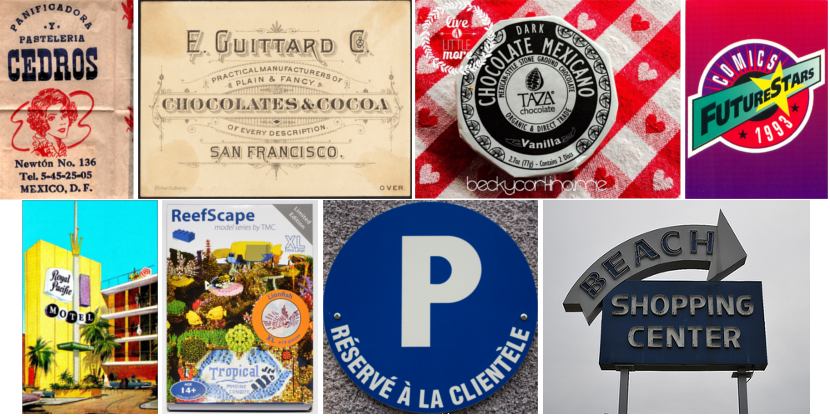
\includegraphics[width=\textwidth]{obrazky/Dataset_ctw.png}
    \caption{Sample images of SCUT-CTW1500 dataset.}
    \label{Im:Dctw}
\end{figure}

\subsection*{KAIST Scene Text Database}

This dataset contains 3000 images of photographed text. It can be divided into three major categories -- text of Korean language, English language and mixed languages. As I concentrate on text in latin script in this paper further information relates to the English language dataset. The number of images is then reduced to less than four hundred images. Figure \ref*{Im:Dkaist} shows few samples of this dataset. Photographed objects are mostly shop banners or parts of magazine front pages. Photographs were either taken by a high-resolution digital camera or a low-resolution mobile phone camera.\cite{kaist} Each photography has a ground truth description and a bitmap image. In the bitmap file only text is highlighted (by white or red color) and everything else apart from text is set as black. Ground truth files are in XML format and includes a name of an image, its resolution and bounding box for each word and also a bounding box for each letter of the word.

To use this dataset for testing and training the XML ground truth needed to be converted to string and int values. I wrote a parser, that combines letters to form a word that is within a given bounding box. I changed the notation of bounding boxes from one coordinate, width and height attributes to two top left and bottom right coordinates. The name of the parsing function is \texttt{read\_gt\_kaist}.

Unfortunately this dataset has few errors in filenames of corresponding files or in the content of XML files. Usually these are only typos, however they prevent automatic preprocessing of dataset. Due to this problem these mistakes need to be found and  manually corrected. Also there is a small number of ground truth XML file with fully missing data. 
Despite these shortcomings this dataset is useful because of the bitmap files. This allows to compare results of both images affected by shooting conditions and images dependent only on font and position.

\begin{figure}[hbtp]
    \centering
    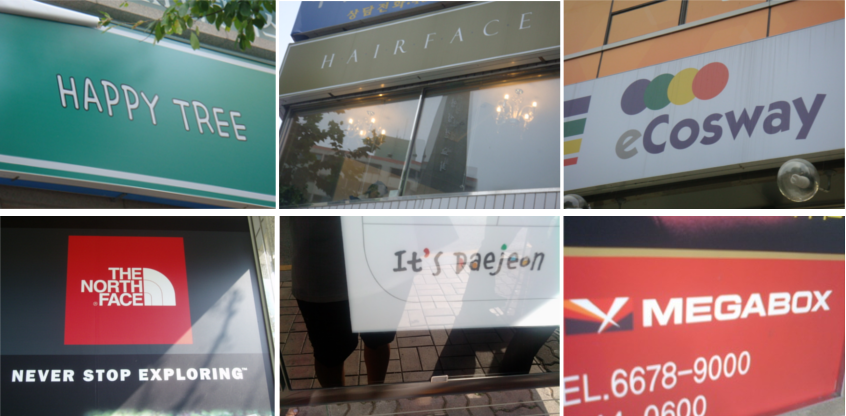
\includegraphics[width=\textwidth]{obrazky/Dataset_kaist.png}
    \caption{Sample images of KAIST Scene Text Database dataset.}
    \label{Im:Dkaist}
\end{figure}

\subsection*{Born-Digital Images}

Born-Digital Images contains data of images with text that can be found on various websites. Samples of this dataset can be found is in Figure \ref*{Im:Dbd}. There are mostly advertisements, company logos or website headers. Such pictures cannot be classified neither as real scene dataset, neither as synthetic one. On one hand  this dataset shares with scene datasets the variability in font styles and sizes, different text orientations and complex colour placement. On the other hand it differs in size because low resolution is significant in smooth and fast loading on websites. Also no noise is present due to lighting conditions. Geometrical deformations that result when capturing a real scene with camera also do not appear here. However compression to lower resolution can lead to artifacts and aliasing. In general we can say that letters are more clearly visible than in photographed text as easy readability is crucial in successful advertising.\cite{born-digital1}

The dataset is available for download from the website of Robust Reading Competition. First version was published in 2011 and revised two years later, it contains separate dataset for text localization, segmentation and then for word recognition. In 2015 they published an end-to-end dataset with ground truth for all tasks. The dataset is split in training and testing data. However, ground truth for testing data contains only a possible vocabulary of words in images and no coordinates. This might be due to the fact that the competition might be still ongoing or there was not a sufficient demand for complete ground truth. As for training data, each image has a corresponding TXT file with coordinates of four vertices of bounding rectangle and a word. Text lines are separated and the text within rectangle is always one word. Extracting ground truth is done in the function \texttt{read\_gt\_bd} and unlike preceding datasets there was no parsing needed, only read the desired values from a file. Unfortunately, there are quite a few missing words, usually words that have two or less characters. This can affect the evaluation when the model finds such a short, missing word.\cite{born-digital1}

\begin{figure}[hbtp]
    \centering
    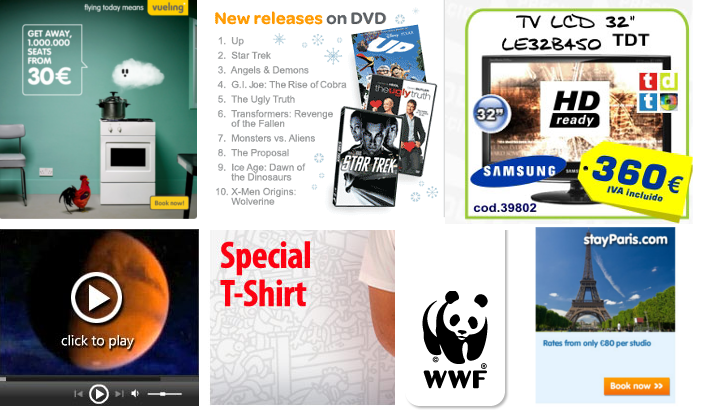
\includegraphics[width=\textwidth]{obrazky/Dataset_born-digital.png}
    \caption{Sample images of Born-Digital Images dataset.}
    \label{Im:Dbd}
\end{figure}


\subsection*{Vienna City Poster Dataset}

The Vienna City Library possesses a collection of 350,000 poster images. A sample of the collection was provided by the organization to the Technical University of Vienna for research purposes. It consists of 5050 images. From these images we manually labeled 257 images and created a testing dataset. Sample of the dataset is in Figure \ref{Im:Dvienna}. As it can be seen from the example images, the dataset includes mainly posters with German language, though few images have words in English or Czech.

\begin{figure}[hbtp]
    \centering
    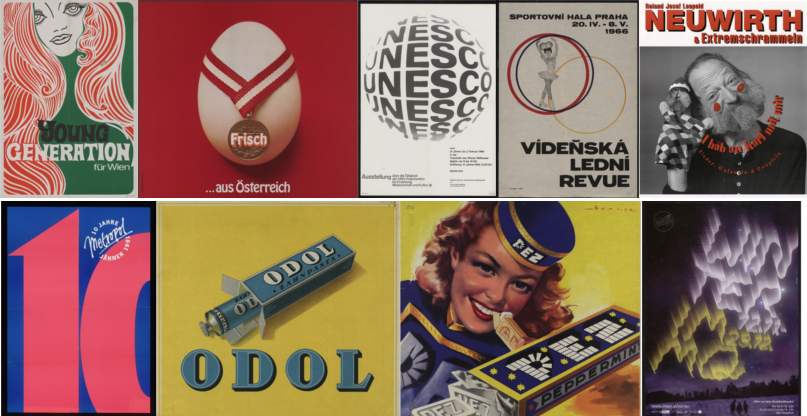
\includegraphics[width=\textwidth]{obrazky/Dataset_vienna.png}
    \caption{Sample images of Vienna City Poster Dataset.}
    \label{Im:Dvienna}
\end{figure}


The posters have neither the characteristic of a scanned text documents, neither of scene images. They are most similar to born digital images. However for the posters is typical one thing -- a part of the text is large relative to the image size and another part is tiny. The huge text is usually a brand or product name or a name of an event. The small text is the name of the author of the poster or the printer where the posters was printed. Both of these texts are a challenge for an OCR engine, because large letters are misinterpreted as objects and the height of the tiny ones is not bigger then twenty pixels and letters are often blurred. Middle-sized text also appears in the posters and is generally well recognized.

Due to the presence of the small text. All images in the dataset need  to be in the original resolution. The bigger side is always 4096 pixels. This leads to a large dataset even when the number of images is less then three hundred. A single JPG image has approximately 4 Megabytes. A PNG image in the dataset has about 20 Megabytes. To reduce the final size of the dataset I decided to convert the PNG files to JPG\footnote{For converting the images I used the console application ImageMagick, with the command \newline \tn{for f in *.png ; do convert "\$f" "../alljpg/\$\{f\%.*\}.jpg" ; done}.}. The final dataset of JPG images is 1.1 GB large, before it was 2.8 GB. The high resolution of images makes demands on the hardware when working with the dataset and makes it impossible to run on machines with insufficiently large computing memory.

The annotation tool used for labeling the selected posters is called Aletheia from the PRiMA Research\footnote{More information available at https://www.primaresearch.org/tools/Aletheia}. The program can be downloaded for Windows operating system, it offers both Lite and Pro version. A free one month trial is offered or for academic use the PRiMA Research gives an extended license. Using this tool we labeled every separate word or group of letters (such as poster identification number) found in an image on the selected posters. Words that were forming a text line, were afterwards labeled as a text line (single word is a text line consisting of one word). Individual characters were not labeled. Bounding boxes for both words and text lines are rectangles, even for curved text. Word bounding boxes were drawn pixel precise with the intention of no margin between the box and the word. Aletheia software produces a XML file with PRiMA Research tags, example for the image P-2151.jpg is in the code below and in Figure \ref{Im:aletheia} is a graphical representation of this XML file.

\begin{lstlisting}[label=lst:xml]
<?xml version="1.0" encoding="UTF-8"?>
<PcGts xmlns="http://schema.primaresearch.org/PAGE/gts/pagecontent/2019-07-15" xmlns:xsi="http://www.w3.org/2001/XMLSchema-instance" xsi:schemaLocation="http://schema.primaresearch.org/PAGE/gts/pagecontent/2019-07-15 http://schema.primaresearch.org/PAGE/gts/pagecontent/2019-07-15/pagecontent.xsd">
<Creator></Creator>
<Created>2022-03-14T11:42:27</Created>
<LastChange>2022-03-14T11:42:27</LastChange></Metadata>
<Page imageFilename="P-2151.jpg" imageWidth="2524" imageHeight="4096">
<TextRegion id="tempReg357564684568544579089">
<Coords points="0,0 1,0 1,1 0,1"/>
<TextLine id="l4">
<Coords points="264,2496 264,2810 2301,2810 2301,2496"/>
<Word id="w10">
<Coords points="264,2496 264,2810 2301,2810 2301,2496"/>
<TextEquiv>
<Unicode>GENERATION</Unicode></TextEquiv></Word>
<TextEquiv>
<Unicode>GENERATION</Unicode></TextEquiv></TextLine>
...
\end{lstlisting}


\begin{figure}[hbtp!]
    \centering
    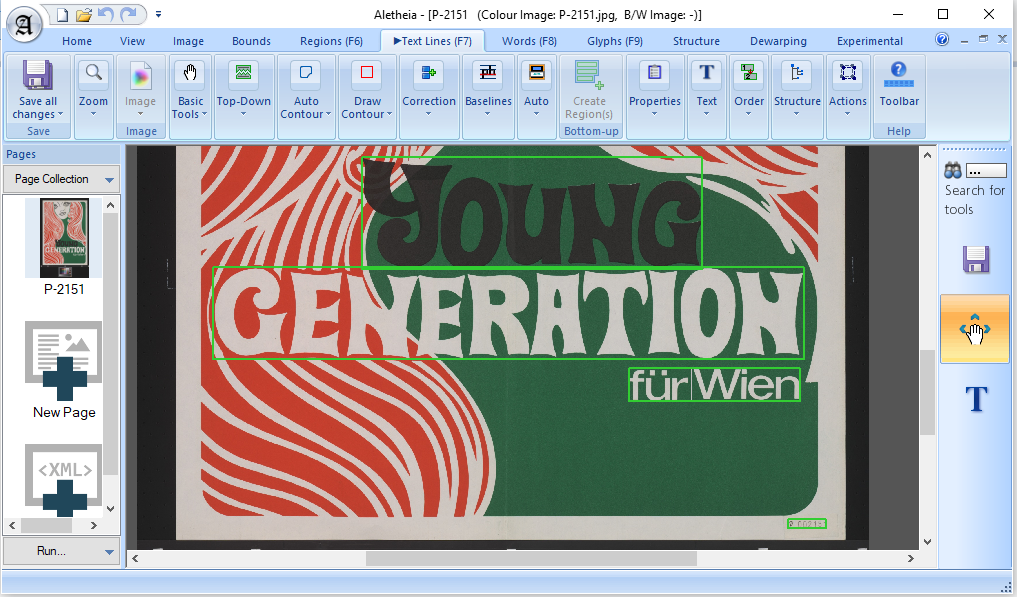
\includegraphics[width=\textwidth]{obrazky/aletheiaim.png}
    \caption{Image P-2151.jpg in the labeling software Aletheia. Green boxes sourrounds ground truth text lines.}
    \label{Im:aletheia}
\end{figure}








% ------------------------------- Implementation -----------------------------

\section{Implementation}
\label{sec:implement}

In this section I briefly described the structure of the experiment scripts and the function used inside them.

I wrote all testing scripts and auxiliary functions in Python programming language. The scripts were written as Jupyter Notebook environment and saved in the corresponding file format \texttt{.ipynb}, lately these notebooks were saved as \texttt{.py} Python scripts. The set of utility functions is located in a file called \texttt{utils.py}. All experiments were run within Google Colaboratory\footnote{Google Colaboratory (Colab for short) is an product from Google Research. It allow Google users to write and execute python code within a web browser using a remote computer and its computing power. In the free version of Colab the computational resources are limited and vary over time due to the demands of other users. The product is available at \url{https://colab.research.google.com/}.} which provides a 12 GB RAM and a GPU Nvidia K80 with 12 GB memory.

In the experiments I have chosen three methods to be tested, namely, Tesseract, EasyOCR and keras-ocr. Each of them has corresponding Python package. For Tesseract I tried two approaches, one with pure Tesseract and another with CRAFT detection tool followed by Tesseract recognizer. 

\subsection{Script Description}

There are four scripts for the tested methods. Each script begins with downloading required packages, that are not already installed in Google Colab environment. This is followed by importing packages to the environment. Then Google Drive is mounted, because that is where image datasets are stored and where is located a file with utility functions. After that the utility functions can be imported, too.

The next stage is dataset loading. Each dataset is loading separately because tests are performed gradually for each dataset within each method. Images and respective ground truths are loaded and saved in variables. The list of image and text data are sorted so that corresponding data have the same indices.

Another step is the prediction. During this phase models are loaded and detection and recognition parameters specified. 

Then metrics are computed. First the predictions are arranged into a same format. Then intersection over union metric for bounding boxes is computed and character error rate for comparing predicted and original texts. Averages of these metrics throughout an image are made for each image and these results are saved. Optionally one can save an image with the original image and bounding boxes and annotations drawn over it.

The pipeline can be summarized in a set of steps.
\begin{enumerate}
    \item Installation of packages that are not in the default Google Colab setting.
    \item Importing dependencies for the project including custom utility functions from \texttt{utils.py}.
    \item Google Drive of the user that runs Google Colab is mounted. (Authentication is needed)
    \item Image files and ground truth files are loaded. Ground truth is converted from files to tuple of string and integer coordinates.
    \item If desired a short preprocessing of images is done (grayscale, Otsu thresholding).
    \item Setup of parameters for OCR.
    \item Model loading.
    \item Prediction.
    \item Conversion of prediction to a unified format (List of tuples of string and integer coordinates for each image, then joined to a list, which contains prediction for all images.)
    \item Computation of evaluation metrics IoU an CER.
    \item Saving and visualizing results.
\end{enumerate}


\subsection{Function Description}
In the rest of this chapter the description of testing Python scripts is provided as well as comment on functions used in testing scripts. Note that int he following function definitions respective docstrings are omitted as they provide similar information as the descriptions, but in a 	briefer version.    

% -------------------------- XML parsing -------------------------- 
\subsubsection*{Functions for Extracting Ground Truth}

I created the following functions in order to extract ground truth information from  text files -- in most cases XML files. Each dataset unfortunately uses a different form of annotations. The styles differ in order of data, tag names, even in type of the recorded data (sometimes individual characters and their position is written or information about curvature). For XML parsing I utilized the The ElementTree XML API, which is imported as xml.etree.ElementTree. Information in XML files is stored in a tree where individual values can be accessed gradually using tags and their attributes.

All functions return annotations in the following format :
\newline \tn{(label, [[top left X, top left Y], [bottom right X, bottom right Y]])}, a tuple of label and bounding rectangle coordinates in an array. 
If the images in the dataset were scaled then coordinates in annotations need to be scaled with same ratio. This ratio can be passed as a function argument and is default to one.

\begin{lstlisting}[caption=read\_gt\_ctw\_test]
def read_gt_ctw_test(data, scaling_ratio=1):
    # one line = one bounding polygon : list of coordinates, each separated by commas, last is the text inside 
    # there are #### before each text, two additional ## no text recognized

    annotations = []
    with open(data, "r") as file:
        for line in file:
            line = line.rstrip('\n')
            text = line.split("####")
            label = text[-1]
            coordinates = text[0].split(",")[:-1]
            c = [int(i) for i in coordinates]
            minX = min(c[::2])*scaling_ratio
            maxX = max(c[::2])*scaling_ratio
            minY = min(c[1::2])*scaling_ratio
            maxY = max(c[1::2])*scaling_ratio

            bbox_coords = np.array( [[minX, minY], [maxX, maxY]] )
            annotations.append((label, bbox_coords))

    return annotations
\end{lstlisting}

The function \tn{read\_gt\_ctw\_test} reads TXT files that contains the annotations for testing part of the SCUT-CTW1500 dataset.


\begin{lstlisting}[caption=read\_gt\_ctw\_train]
def read_gt_ctw_train(xml_file, scaling_ratio=1):
    gt = []

    tree = ET.parse(xml_file)
    root = tree.getroot()

    # get values in this order: height, left coordinate, top coordinate, width
    for i, bbox in enumerate(root[0].findall('box')):
        # create list of integers with bounding box values, sort by attribute name
        # in case in different document there is a different order of attributes
        bbox_integer = [int(val) for key, val in sorted(bbox.attrib.items(), key = lambda el: el[0])]
        
        # calculate bottom coordinate of bounding rectangle x+width, y+height
        x_right= int((bbox_integer[1] + bbox_integer[3]) * scaling_ratio)
        y_bottom = int((bbox_integer[2] + bbox_integer[0]) * scaling_ratio)
        x_left = int(bbox_integer[1] * scaling_ratio)
        y_top = int(bbox_integer[2] * scaling_ratio)

        bbox_coords = np.array([[x_left, y_top], [x_right, y_bottom]])

        # get label
        label = root[0][i].find('label').text

        # create list of labels and corresponding bounding boxes
        gt.append((label, bbox_coords))

    return gt
\end{lstlisting}

The function \tn{read\_gt\_ctw\_train} reads the annotations from  XML files for training part of the SCUT-CTW1500 dataset.

\begin{lstlisting}[caption=read\_gt\_kaist]
def read_gt_kaist(xml_file, scaling_ratio=1):
    gt = []

    tree = ET.parse(xml_file)
    root = tree.getroot()

    # some files has images as root tag, 
    # some image as root tag (one tree layer (tag images) is missing)
    try:
        image_tag = root[0][2]
    except IndexError:
        image_tag = root[2]

    # get values in this order: height, width, x (left) coordinate, y (top) coordinate
    for i, bbox in enumerate(image_tag.findall('word')):
        # create list of integers with bounding box values, sort by attribute name
        # in case in different document there is a different order of attributes
        bbox_integer = [int(val) for key, val in sorted(bbox.attrib.items(), key = lambda el: el[0])]
        
        # calculate bottom coordinate of bounding rectangle x+width, y+height
        x_right= int((bbox_integer[2] + bbox_integer[1]) * scaling_ratio)
        y_bottom = int((bbox_integer[3] + bbox_integer[0]) * scaling_ratio)
        x_left = int(bbox_integer[2] * scaling_ratio)
        y_top = int(bbox_integer[3] * scaling_ratio)

        bbox_coords = np.array([[x_left, y_top], [x_right, y_bottom]])

        # get label
        label = ""
        for char in image_tag[i].findall('character'):
            ch = char.get('char')
            label += ch
        # create list of labels and corresponding boundin boxes
        gt.append((label, bbox_coords))

    return gt
\end{lstlisting}

The function \tn{read\_gt\_kaist} extract annotations from XML files with labels for KAIST Scene Text dataset.

\begin{lstlisting}[caption=read\_gt\_bd]
def read_gt_bd(data, scaling_ratio=1):
    annotations = []

    with open(data, "r", encoding='utf-8-sig') as file:
        for line in file:
            line = line.rstrip('\n')
            text = line.split(",")
            bbox_coords = np.array(
                [[int(text[0])*scaling_ratio, int(text[1])*scaling_ratio], 
                [int(text[4])*scaling_ratio, int(text[5])*scaling_ratio]])
            annotations.append((text[-1], bbox_coords))

    return annotations

\end{lstlisting}

Annotations for the Born-Digital dataset are stored in simple TXT file, where there are only four coordinates of the four corners of each bounding rectangle and a word within the rectangele. These values are processed by the function \tn{read\_gt\_bd}.

\begin{lstlisting}[caption=read\_gt\_wien]
def read_gt_wien(xml_file, scaling_ratio=1, resized_previously=False):
    # poster dataset
    # returns labels in a tuple - first contains coordinates (8 numbers), second word (string)

    tree = ET.parse(xml_file)
    root = tree.getroot()
    image_width = root.find('{http://schema.primaresearch.org/PAGE/gts/pagecontent/2019-07-15}Page').get('imageWidth')

    if resized_previously:
        scaling_ratio = scaling_ratio / int(image_width)

    root.iter('{http://schema.primaresearch.org/PAGE/gts/pagecontent/2019-07-15}TextRegion')

    annotations = []
    for word in root.iter('{http://schema.primaresearch.org/PAGE/gts/pagecontent/2019-07-15}Word'):
        coordinates = word.find('{http://schema.primaresearch.org/PAGE/gts/pagecontent/2019-07-15}Coords').get('points')
        text = word.find('{http://schema.primaresearch.org/PAGE/gts/pagecontent/2019-07-15}TextEquiv')
        # extract only top left and bottom right coordinates and apply scale
        coords = coordinates.split(" ")
        topL = coords[0].split(",")
        bottomR = coords[2].split(",")
        bbox_coords = np.array(
                    [[int(int(topL[0])*scaling_ratio), int(int(topL[1])*scaling_ratio)], 
                    [int(int(bottomR[0])*scaling_ratio), int(int(bottomR[1])*scaling_ratio)]])
        annotations.append((text[0].text, bbox_coords))

    return annotations
\end{lstlisting}

The function \tn{read\_gt\_wien} takes the label and coordinate values form a XML files for the Vienna City Poster Dataset. The XML files produced by the software Aletheia are in a format created by PRiMA Research. When going through the XML tree an information about the research organization is embodied in the tag names.

\subsubsection*{Functions for Editing Images}

\begin{lstlisting}[caption=image\_text\_crop]
def image_text_crop(images, filenames, ground_truth, one_file=True, result_folder='./results', skip_longer_than=40):
    # test if there are not more gts than images
    # else the for loop will never get to those exceeding image count
    gt_length = len(ground_truth)
    if len(images) > gt_length:
        images = images[:gt_length]

    if not os.path.isdir(result_folder):
        os.mkdir(result_folder)

    all_texts = []
    for i, img in tqdm(enumerate(images)):
        name, ext = os.path.splitext(filenames[i])

        # count regions in one image - used for file naming purposes
        region = 1
        
        for text, bbox in ground_truth[i]:
            if text is None:
                continue
            if len(text) > skip_longer_than:
                continue
            # select image within coordinates (bbox)
            cropped = img[bbox[0,1]:bbox[1,1], bbox[0,0]:bbox[1,0]]

            # create image file:
            # name in format "original-00region.ext"
            new_name = name + '-' + str(region).zfill(3)
            
            if np.size(cropped):
                cv.imwrite(os.path.join(result_folder, new_name + ext), cropped)
                # create  text annotation file(s)
                if one_file:
                    all_texts.append(new_name + ext + '\t' + text)
                else:
                    # one file for each image with word
                    all_texts.append(new_name + ext + '\t' + text)
                    with open(os.path.join(result_folder, new_name + '.gt.txt'), 'w') as f:
                        f.write(text)
                region += 1

    if one_file:
        with open(os.path.join(result_folder, 'gt.txt'), 'w') as f:
            for line in all_texts:
                f.writelines(line+'\n')

    return all_texts
\end{lstlisting}

The function \tn{image\_text\_crop} crops and saves images based on bounding boxes provided in ground truth for each text region in an image. This is done for all images in \tn{images} list. Also a text file is created with a corresponding text annotation. The name of the resulted file bears the original image name and a number is attached for each text region. The boolean parameter \tn{one\_file} allows to save ground truths only to a single file. Each line consists then of the name of the cropped image and its annotation. The parameter \tn{skip\_longer\_than} skips ground truths that have more characters than stated, because some OCR tools (such as keras-OCR) does not support long strings.

\begin{lstlisting}[caption=shrink\_all]
def shrink_all(images, width):
    scaled = []
    
    for image in images:
        if image.shape[1] > width:
            ratio = width / image.shape[1]
            height = int(image.shape[0] * ratio)
            new_size = (width, height)  
            scaled.append(cv.resize(image, new_size, interpolation=cv.INTER_AREA))
        else:
            scaled.append(image)
    return scaled    
\end{lstlisting}

The function \tn{shrink\_all} returns a list of resized images to a given width. Images already smaller than width are kept unaffected. The resizing aspects ratio.


\begin{lstlisting}[caption=bounding\_rectangle]
def bounding_rectangle(coordinates):
    x, y = zip(*coordinates)

    return np.array([[int(min(x)), int(min(y))], [int(max(x)), int(max(y))]])
\end{lstlisting}

The function \tn{bounding\_rectangle}
Returns top left and bottom right coordinates of a rectangle, that is circumscribed to a polygon defined by coordinates. These are obtained from predictions for each text region.

\subsubsection*{Functions for Computing Metrics}

% -------------------------- IoU --------------------------  

\begin{lstlisting}[caption=iou]
def iou(pred_box, gt_box):
    # find intersection rectangle coordinates
    x_left = max(pred_box[0][0], gt_box[0][0])
    x_right = min(pred_box[1][0], gt_box[1][0])
    y_top = max(pred_box[0][1], gt_box[0][1])
    y_bottom = min(pred_box[1][1], gt_box[1][1])

    if x_right < x_left or y_bottom < y_top:
        return 0
    
    # compute intersection area
    intersection = (x_right - x_left) * (y_bottom - y_top)

    # compute union area
    pred_area = (pred_box[1][0] - pred_box[0][0]) * (pred_box[1][1] - pred_box[0][1]) 
    gt_area = (gt_box[1][0] - gt_box[0][0]) * (gt_box[1][1] - gt_box[0][1]) 
    union  = pred_area + gt_area - intersection

    # return iou
    return  intersection/union

\end{lstlisting}

The function \tn{iou} computes intersection over union of two bounding boxes, as defined in \ref*{sec:eval}. Both input parameters have to contain top left and bottom right coordinates of a bounding box rectangle.

\begin{lstlisting}[caption=iou\_image]
def iou_image(pred_boxes, gt_boxes):
    ious = []

    # have to determine which prediction bounding box contains same (similar) 
    #  text region as ground truth bounding box
    # find and save the best iou for a prediction box and gt box
    for pred_ind, pred in enumerate(pred_boxes):
        max_iou = 0
        max_ind = 0
        for gt_ind, gt in enumerate(gt_boxes):
            iou_value = iou(pred, gt)
            if (iou_value > max_iou):
                max_iou = iou_value
                max_ind = gt_ind

        # match words from prediction and ground thruth (indices)     
        ious.append((max_iou, pred_ind, max_ind))

    return ious

\end{lstlisting}

The function \tn{iou\_image} computes intersection over union for all text regions in one image.
Each parameter shall contain a list of two coordinates - (top left, bottom right) of a bounding box rectangle.
Returns a list of tuples - each tuple consists of the highest iou value (thus having the biggest overlap), the index of predicted bounding box and  the index of ground truth bounding box. The indices are taken from the given lists of bounding boxes or ground truths belonging to one particular image.

\begin{lstlisting}[caption=group\_text]
def group_text(lst):
    grouped = []
    key = lambda x: x[2]

    for k, g in itertools.groupby(sorted(lst, key=key), key):
        list_data = list(zip(*g))
        grouped.append((sum(list_data[0]), list_data[1], k))

    return grouped
\end{lstlisting}

The function \tn{group\_text} is a utility function for matching corresponding strings in a list. The list that is passed as an argument is a list of tuples of IoUs returned from the function \tn{iou\_image}. First for each ground truth bounding box, which is determined by the ground truth index (in this case the third element of the tuple) and it is used as a key. The returned tuple consists of a sum of IoUs, a list of indices of predicted bounding boxes and ground truth index.

% -------------------------- Text Comparision -------------------------- 


\begin{lstlisting}[caption=compare\_text\_cer]
def compare_text_cer(text, special_characters=False, case_sensitive=False, spaces=True, split=True):
    text_gt, text_pred = text
    # remove special characters and case sensitivity if necessary
    if not spaces:
        text_gt = "".join(char for char in text_gt if (char.isalnum()))
        text_pred = "".join(char for char in text_pred if (char.isalnum()))
    elif not special_characters:
        text_gt = "".join(char for char in text_gt if (char.isalnum() or char.isspace()))
        text_pred = "".join(char for char in text_pred if (char.isalnum() or char.isspace()))
    if not case_sensitive:
        text_gt = text_gt.lower()
        text_pred = text_pred.lower()
    
    corresponding_words = []

    if split:
        words_gt = text_gt.split(" ")
        words_pred = text_pred.split(" ")

        # list of words that are corresponding (based on levenshtein distance)
        # and cer value. (=tuple of three elements)
        # for every predicted word find its corresponding gt wordle
        for word_pred in words_pred:    
            min_dist = (1000, (0, 0))
            min_gt_word = ""                  
            for word_gt in words_gt: 
                l_dist = levenshtein_distance(word_gt, word_pred)
                if l_dist[0] < min_dist[0]:
                    min_dist = l_dist
                    min_gt_word = word_gt
            # count normalized cer (the result will be from 0 to 1), 1 is the worst
            # for computation we devide Levenshtein dist. by sum 
            # of the length of the word and count of insertions performed
            if len(min_gt_word) > 0 and len(word_pred) > 0:
                cer = min_dist[0] / (len(min_gt_word) + min_dist[1][2])
            else:
                cer = 1
            corresponding_words.append((min_gt_word, word_pred, cer))

        # no split of words    
    else:
        l_dist = levenshtein_distance(text_gt, text_pred)

        if len(text_gt) > 0 and len(text_pred) > 0:
            cer = l_dist[0] / (len(text_gt) + l_dist[1][2])
        else:
            cer = 1
        corresponding_words.append((text_gt, text_pred, cer))

    return sorted(corresponding_words)
\end{lstlisting}

The function \tn{compare\_text\_cer} returns a sorted list of corresponding words. Each pair of corresponding words is represented as a tuple of ground truth string, predicted string and a CER value. The first parameter have to be a tuple of a single ground truth string and a predicted string. The argument \tn{special\_characters} ignores all characters except alphanumeric characters and space when \tn{False}. This is applied to both predicted and ground truth strings. When the argument \tn{case\_sensitive} is \tn{False} then all texts are set to lowercase. The \tn{spaces} parameter allows only alphanumeric characters and all spaces are removed. The last one of arguments is \tn{split} and it is used optionally depending on the OCR engine and on dataset. When \tn{True}, strings from ground truth and prediction are split with space used as a separator. Then the Levenshtein distance is computed for each pair of ground truth and predicted word. The best one is chosen for each predicted word and returned together with the two closest words. In case of no split, the Levenshtein distance is computed directly for the strings in the original tuple \tn{text}. It is recommended to use split when the OCR model tends to detect words that belongs to each other as separate words and ground truth marks them as a text line with multiple words. Or when ground truth is one-word and model predicts strings with multiple words together.

The function \tn{levenshtein\_distance} computes the Levenshtein distance (definition can be found in subsection \ref*{sec:eval}). The implementation is taken from a console application called xer. The code is available from \url{https://github.com/jpuigcerver/xer/blob/master/xer}. It returns a tuple of counts of the three performed operations --  substitution, deletion, insertion.

\subsubsection*{Other Functions}

\begin{lstlisting}[caption=correct]
def correct(string, char_mistakes):
    """
    Find defined mistake in a string and replace it with defined correction.
    Returns corrected string.
    """correct
    
    for oldchar, newchar in char_mistakes:
        string = string.replace(oldchar, newchar)

    return string
\end{lstlisting}   

\begin{lstlisting}[caption=correct\_german,label={lst:correctgerman}]    
def correct_german(text):    
    # For all texts correct these mistakes
    text = correct(text, [('iu','in'),('LN','IN')])

    length = len(text)

    # ! shall be at the end of the text, if not it is probably the letter I
    if length > 1 and text.find('!') != length-1:
        text = text.replace('!','I')

    # For longer texts other mistakes can be corrected
    if length > 2:

    char_mistakes = [('{','f'),('$','S'),('[','L'),('/','I'),('|','I'),('ETN','EIN'),
                    ('CE','GE'),('GH','CH'),('GU','QU'),('gu','qu'),('IZ','TZ'),
                    ('UNO','UND'),('uno','und'),('Wlen','Wien'),('wlen','wien')]
    text = correct(text, char_mistakes)

    # No Y at the begining of german words
    if text.find('Y')==0:
        text = 'V' + text[1:]


    # Characters that do appear in text sometimes, but usually alongside numbers
    # not if there are no numbers 
    char_difficult = [('1','I'),('{euro sign}','E')]
    for old, new in char_difficult:
        if text.find(old) is not -1 and text.replace(' ','').replace(old,'').isalpha():
            text = text.replace(old,new)

    if text.find('(') is not -1 and text.find(')') is -1:
        text = text.replace('(','C')

    spaces = text.count(' ')
    if  spaces > length/2 - 2:
        text = text.replace(' ','')
            
    return text
\end{lstlisting}   

The function returns corrected text based on typical German language syllables  and common mistakes caused by optical character recognizers.

% -------------------------- Testing Scripts -------------------------- 
\subsubsection*{Functions Used in Testing Scripts}

For each testing method there is a function called \tn{get\_predicted\_\{method\_name\}} where the format that is returned by a particular method is converted to a specific format. This format is a tuple of \tn{(text, [upper left coordinates, bottom right coordinates])}. It is the same format as is used for ground truth.

Two following functions manipulate with the IoU and CER scores.

\begin{lstlisting}[caption=get\_iou\_cer]
def get_iou_cer(ground_truth, predicted, special_chars=False, case_sensitivity=False, split=False):
    iou_images = []
    cer_images = []
    n_imgs = len(predicted)
    
    # loop through images:
    for i in range(n_imgs):
        # separate list on columns (iterate through tuples in the list)
        if len(predicted[i]) and len(ground_truth[i]):
            predicted_cols = list(zip(*predicted[i]))
        else:
            iou_images.append(None)
            cer_images.append(None)
            continue
        ground_truth_cols = list(zip(*ground_truth[i]))

        # take only coordinate arrays from list for each images
        pred_boxes = predicted_cols[1]
        gt_boxes = ground_truth_cols[1]
        iou_from_image = iou_image(pred_boxes, gt_boxes)
        iou_text_regions = group_text(iou_from_image)
      
        # take only labels for each image
        pred_labels = predicted_cols[0]
        gt_labels = ground_truth_cols[0]

        # compare corresponding labels
        # comparison is a list of all text regions on one image
        comparision = []

        for observation in iou_text_regions:
            gt_ind = observation[-1]
            pred_ind = observation[1]
            predicted_text = " ".join([pred_labels[i] for i in pred_ind])

            if split:
                gt_text = " ".join([i for i in gt_labels if i is not None])
            else:
                gt_text = gt_labels[gt_ind]

            if gt_text is None or predicted_text is None:
                continue
                
            gt_pred_text = (gt_text, predicted_text)

            # comparision for one text region (on one image)
            comparision.append((compare_text_cer(gt_pred_text, special_characters=special_chars, case_sensitive=case_sensitivity, split=split)))

        iou_images.append((iou_text_regions))
        cer_images.append((comparision))

    return iou_images, cer_images
\end{lstlisting}

The function \tn{get\_iou\_cer} returns IoU and CER metric for bounding boxes for all images for each text region detected in an image. Thus there are two tuples with the length of number of images in a dataset.

\begin{lstlisting}[caption=get\_iou\_cer\_average]
def get_iou_cer_average(iou_images, cer_images):
    iou_in_image = []
    cer_in_image = []
    n_imgs = len(iou_images)
    
    for i in range(n_imgs):
        # calculate mean based on results 
        if isinstance(cer_images[i], list):
            length = len(cer_images[i])
            mean_in_regions = average([average(list(zip(*cer_images[i][j]))[2]) for j in range(length) ])
            iou_in_image.append(average(list(zip(*iou_images[i]))[0]))
        else:
            mean_in_regions = None
            iou_in_image.append(None)

        cer_in_image.append(mean_in_regions)
        
    return iou_in_image, cer_in_image
\end{lstlisting}
   
The function \tn{get\_iou\_cer\_average} returns two tuples of average IoU and CER value for each image in dataset.


% -------------------------- Final Visualization -------------------------- 
\subsubsection*{Functions for Final Visualizations}

\begin{lstlisting}[caption=get\_results]
def get_results(filenames, iou_in_image, cer_in_image):
    df_results = pd.DataFrame(list(zip(filenames, iou_in_image, cer_in_image)), columns =['Filename', 'IoU', 'CER'])
    mean_iou = round(df_results['IoU'].mean() * 100, 1)
    mean_cer = round((1 - df_results['CER'].mean()) * 100, 1)
    
    print(f"mean IoU accuracy = {mean_iou}%, mean CER accuracy = {mean_cer}%")
    display(df_results)
    
    return mean_iou, mean_cer, df_results
    
\end{lstlisting}

The function \tn{get\_results} prints returns average IoU and CER for the whole dataset and a dataframe with these metrics for each image.


\begin{lstlisting}[caption=plot\_results]
def plot_results(image, ground_truth, predicted, size=15):
    # Create figure and axes
    figure, ax = plt.subplots(figsize=(size, size))

    # Display the image
    ax.imshow(cv.cvtColor(image, cv.COLOR_BGR2RGB), cmap=plt.get_cmap('gray'))
    ax.axis('off')

    for label, bbox  in ground_truth:
        topleft = bbox[0]
        height = bbox[1,1] - bbox[0,1]
        width = bbox[1,0] - bbox[0,0]

        # create and add rectangle
        rect = patches.Rectangle((topleft), width, height, linewidth=1, edgecolor='g', facecolor='none')
        ax.add_patch(rect)

        # add labels
        ax.text(topleft[0]+width, topleft[1],label,verticalalignment='top', color='g',fontsize=13, bbox=dict(facecolor='g', alpha=0.2, edgecolor='g'))

    for label, bbox  in predicted:
        topleft = bbox[0]
        height = bbox[1,1] - bbox[0,1]
        width = bbox[1,0] - bbox[0,0]

        # create and add rectangle
        rect = patches.Rectangle((topleft), width, height, linewidth=1, edgecolor='r', facecolor='none')
        ax.add_patch(rect)

        # add labels
        ax.text(topleft[0]-2, topleft[1]-5,label,verticalalignment='top', color='r',fontsize=13, bbox=dict(facecolor='r', alpha=0.2, edgecolor='r'))
    
    # smaller white borders
    plt.subplots_adjust(left=0, bottom=0.1, right=1, top=0.9, wspace=0, hspace=0)

    return plt 
\end{lstlisting}

The function \tn{plot\_results} returns a plot with an image and both predicted and ground truth bounding boxes 
and corresponding labels. The ground truths are marked with green color and predictions with red. Objects are drawn using the package matplotlib.

% \subsection{Visualisation}
%  The notebook \tn{results\_visualization}.